%
% $RCSfile: introduction.tex,v $
%
% Copyright (c) 2002-2007. Christian Heller. All rights reserved.
%
% Permission is granted to copy, distribute and/or modify this document
% under the terms of the GNU Free Documentation License, Version 1.1 or
% any later version published by the Free Software Foundation; with no
% Invariant Sections, with no Front-Cover Texts and with no Back-Cover
% Texts. A copy of the license is included in the section entitled
% "GNU Free Documentation License".
%
% http://www.cybop.net
% - Cybernetics Oriented Programming -
%
% Version: $Revision: 1.2 $ $Date: 2007-08-01 13:59:00 $ $Author: christian $
% Authors: Christian Heller <christian.heller@tuxtax.de>
%

\chapter{Introduction}
\label{introduction_heading}
\index{Introduction}

The \emph{Cybernetics Oriented Language} (CYBOL) is an interpretable knowledge
modelling- and programming language. It is very flexible, has a simple syntax
and is easy to learn. Hence, not only classical software designers- and
developers, but also analysts and domain experts may have an interest in CYBOL.

Its simplicity is based on the fact that just one major concept needs to be
understood: that of \emph{Hierarchy}. Well, in fact CYBOL applies it in form of
a \emph{Double Hierarchy}, but is this not very difficult to grasp, as the code
examples later in this document will show.

%
% $RCSfile: theory.tex,v $
%
% Copyright (c) 2002-2007. Christian Heller. All rights reserved.
%
% Permission is granted to copy, distribute and/or modify this document
% under the terms of the GNU Free Documentation License, Version 1.1 or
% any later version published by the Free Software Foundation; with no
% Invariant Sections, with no Front-Cover Texts and with no Back-Cover
% Texts. A copy of the license is included in the section entitled
% "GNU Free Documentation License".
%
% http://www.cybop.net
% - Cybernetics Oriented Programming -
%
% Version: $Revision: 1.1 $ $Date: 2007-08-01 13:59:01 $ $Author: christian $
% Authors: Christian Heller <christian.heller@tuxtax.de>
%

\section{Theory}
\label{theory_heading}
\index{CYBOP}
\index{Theory}

The theory behind CYBOL is called \emph{Cybernetics Oriented Programming}
(CYBOP). It describes the general concepts, software architecture and
development principles that justify the existence of CYBOL. Besides CYBOL as
language, CYBOP suggests the \emph{Cybernetics Oriented Interpreter} (CYBOI).

\begin{figure}[ht]
    \begin{center}
        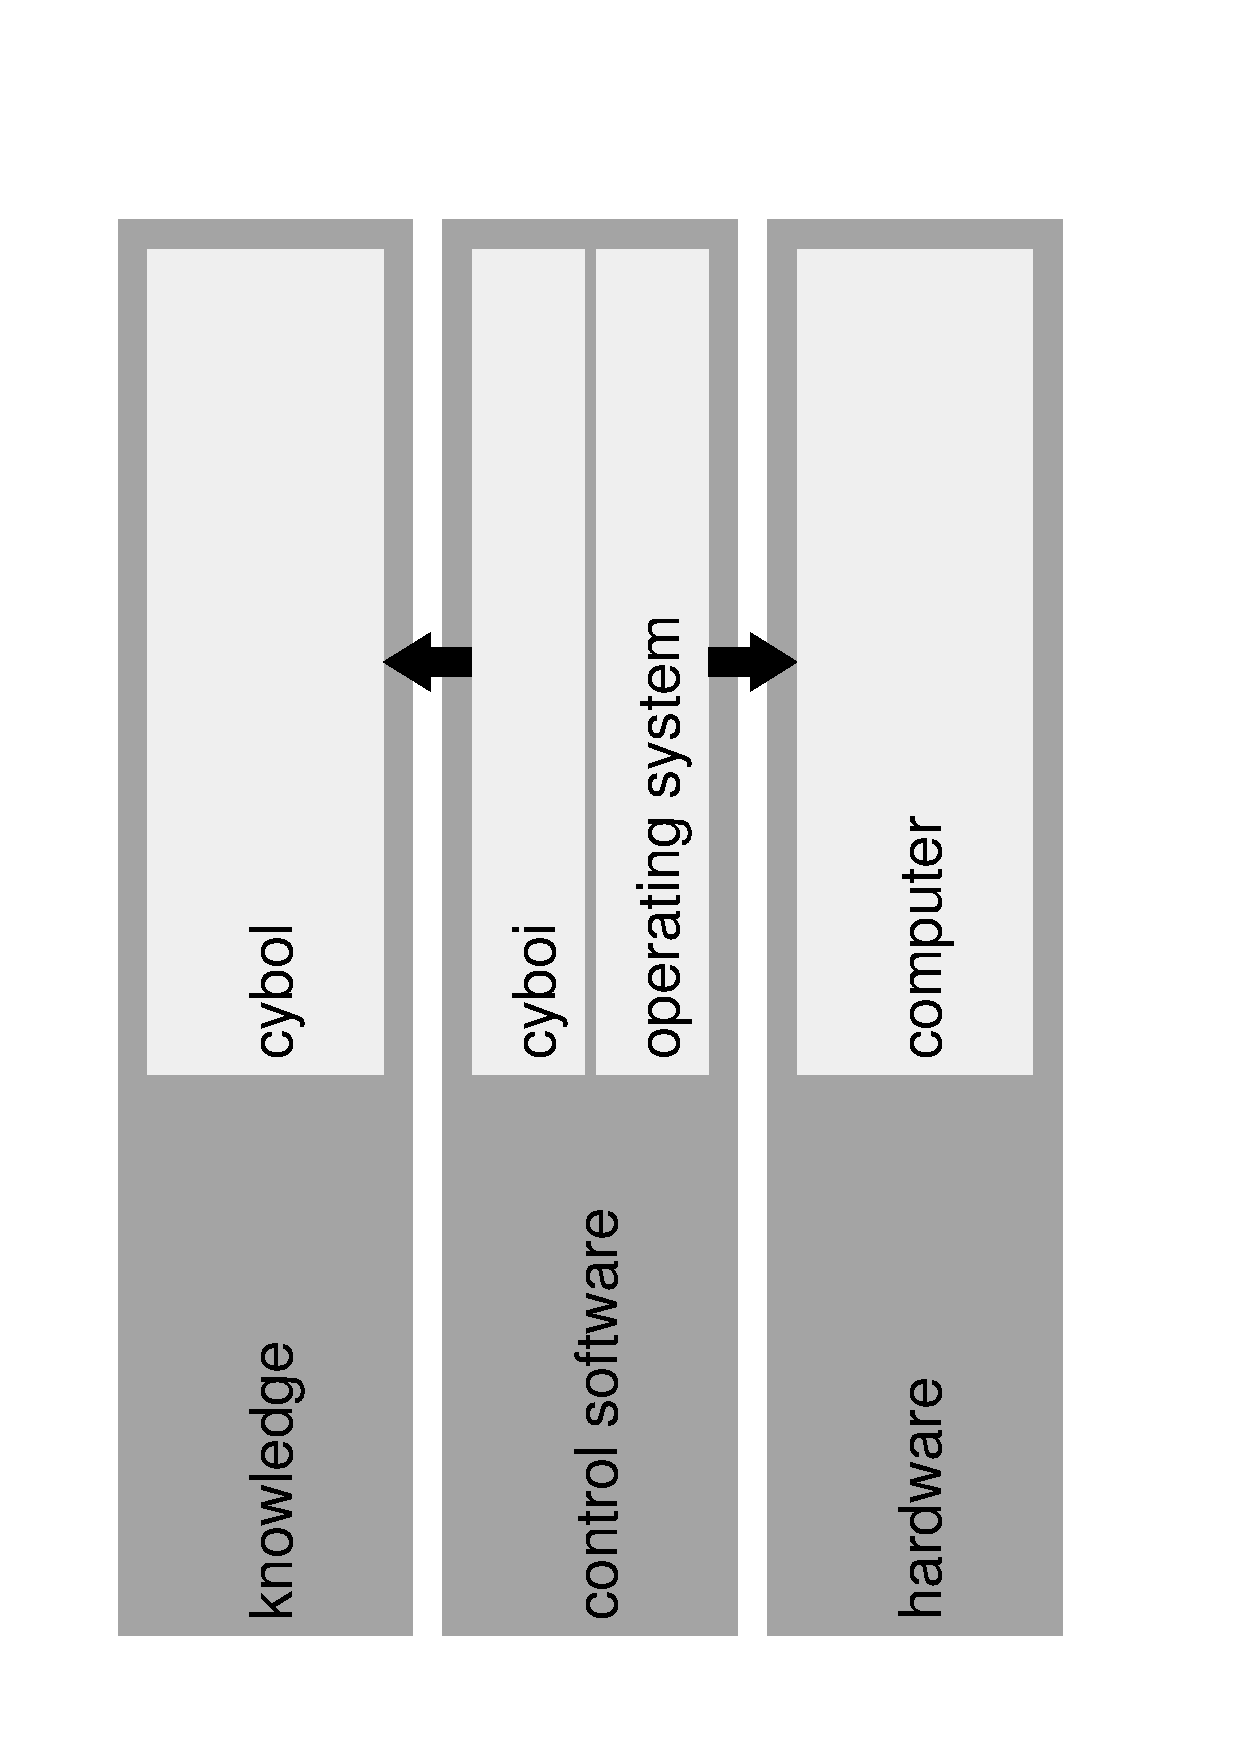
\includegraphics[scale=0.3,angle=-90]{graphics/interpretation.pdf}
        \caption{CYBOL Interpretation}
        \label{interpretation_figure}
    \end{center}
\end{figure}

Considering an overall computer system architecture, \emph{CYBOI} as low-level
software system is situated between the application knowledge existing in form
of \emph{CYBOL} templates and the \emph{Hardware} controlled by an
\emph{Operating System} (OS), as is shown in figure \ref{interpretation_figure}.
CYBOI as \emph{active} system process interprets the \emph{passive} application
knowledge provided in form of CYBOL files.

Design-time knowledge resides in CYBOL \emph{Knowledge Templates} (files).
While being instantiated, it gets transferred into runtime
\emph{Knowledge Models} that reside in a computer's \emph{Random Access Memory}
(RAM).

%
% $RCSfile: analogy.tex,v $
%
% Copyright (c) 2002-2007. Christian Heller. All rights reserved.
%
% Permission is granted to copy, distribute and/or modify this document
% under the terms of the GNU Free Documentation License, Version 1.1 or
% any later version published by the Free Software Foundation; with no
% Invariant Sections, with no Front-Cover Texts and with no Back-Cover
% Texts. A copy of the license is included in the section entitled
% "GNU Free Documentation License".
%
% http://www.cybop.net
% - Cybernetics Oriented Programming -
%
% Version: $Revision: 1.1 $ $Date: 2007-08-01 13:59:00 $ $Author: christian $
% Authors: Christian Heller <christian.heller@tuxtax.de>
%

\section{Analogy}
\label{analogy_heading}
\index{Analogy between CYBOP and Java}
\index{Java-CYBOP Analogy}
\index{CYBOP-Java Analogy}
\index{CYBOI as Virtual Machine}

There are analogies to other systems run by language interpretation. Table
\ref{analogy_table} shows that between the \emph{Java-} and \emph{CYBOP} world.
Both are based on a programming theory, have a language and interpreter, the
latter sometimes being called a \emph{Virtual Machine} (VM).

\begin{table}[ht]
    \begin{center}
        \begin{footnotesize}
        \begin{tabular}{| p{35mm} | p{35mm} | p{35mm} |}
            \hline
            \textbf{Criterion} & \textbf{Java World} & \textbf{CYBOP World}\\
            \hline
            Theory & OOP in Java & CYBOP\\
            \hline
            Language & Java & CYBOL\\
            \hline
            Interpreter & Java VM & CYBOI\\
            \hline
        \end{tabular}
        \end{footnotesize}
        \caption{Analogy between the Java- and CYBOP World}
        \label{analogy_table}
    \end{center}
\end{table}

CYBOI provides low-level, platform-dependent system functionality, close to the
OS, together with a unified knowledge schema which allows CYBOL applications to
be truly portable, well extensible and easier to program, because developers
need to concentrate on domain knowledge only. Since CYBOI may interpret CYBOL
sources \emph{live} at system runtime, without the need for previous compilation
(as in Java), changes to CYBOL sources can get into effect right away, without
having to restart the system.

